
%(BEGIN_QUESTION)
% Copyright 2015, Tony R. Kuphaldt, released under the Creative Commons Attribution License (v 1.0)
% This means you may do almost anything with this work of mine, so long as you give me proper credit

In each of these process control examples, the transmitter produces an increasing signal for an increase in process measurement (level, pressure, temperature, etc.), and the I/P transducer produces an increasing air pressure signal out for an increasing current signal in.  

Your task is to determine the proper action for the process controller, either {\it direct-acting} or {\it reverse-acting}.  Remember, a direct-acting controller produces an increasing output signal with an increasing process variable input.  A reverse-acting controller produces a decreasing output signal for an increasing process variable input.  It is essential for stability that the controller have the correct direction of action!

\vskip 10pt

\noindent
{\bf Example 1:}

$$\includegraphics[width=15.5cm]{i00788x01.eps}$$

\vskip 10pt

\filbreak
\noindent
{\bf Example 2:}

$$\includegraphics[width=15.5cm]{i00788x02.eps}$$

\vskip 10pt

\filbreak
\noindent
{\bf Example 3:}

$$\includegraphics[width=15.5cm]{i00788x03.eps}$$

\vskip 10pt

\filbreak
\noindent
{\bf Example 4:}

$$\includegraphics[width=15.5cm]{i00788x04.eps}$$


\vskip 10pt

\filbreak

A concept familiar to students of electronics is the {\it differential amplifier}, a device built to compare two input signals and generate an output signal proportional to that comparison.  The most common form of differential amplifier is the so-called {\it operational amplifier} or ``opamp'', drawn as a triangle with two inputs labeled ``+'' and ``$-$'' to show the relative influence of each input signal on the output.  A process controller may be thought of as a kind of differential amplifier, sensing the difference between two input signals (the process variable and the setpoint) and generating an output signal proportional to the difference between PV and SP to drive a final control element.

The following process control examples replace the controller symbol with an amplifier symbol.  Your task is to figure out appropriate labels for the amplifier's input terminals (e.g. ``+'' and ``$-$'').  Remember that a controller is defined as being ``direct-acting'' if an increase in PV causes an increase in output and ``reverse-acting'' if an increase in PV causes a decrease in output.  Following opamp labeling, this means the PV input of a direct-acting controller should bear a ``+'' mark while the PV input of a reverse-acting controller should bear a ``$-$'' mark.

$$\includegraphics[width=15.5cm]{i00788x00.eps}$$

\vskip 10pt

\filbreak
\noindent
{\bf Example 5:} {\it Label the PV \& SP amplifier inputs for the correct controller action}

$$\includegraphics[width=15.5cm]{i00788x05.eps}$$

\vskip 10pt

\filbreak
\noindent
{\bf Example 6:} {\it Label the PV \& SP amplifier inputs for the correct controller action}

$$\includegraphics[width=15.5cm]{i00788x06.eps}$$

\vskip 10pt

\filbreak
\noindent
{\bf Example 7:} {\it Label the PV \& SP amplifier inputs for the correct controller action}

$$\includegraphics[width=15.5cm]{i00788x07.eps}$$





\vskip 20pt \vbox{\hrule \hbox{\strut \vrule{} {\bf Suggestions for Socratic discussion} \vrule} \hrule}

\begin{itemize}
\item{} As always, what is more important than arriving at the correct answer(s) is to develop a clear and logical {\it reason} for your correct answers.  Explain the problem-solving technique(s) you used to determine correct controller action in each of these process control examples.
\item{} A powerful problem-solving technique is performing a {\it thought experiment} where you mentally simulate the response of a system to some imagined set of conditions.  Describe a useful ``thought experiment'' for any of these process control loops, and how the results of that thought experiment are helpful to answering the question.
\item{} Explain how to reliably identify the process variable (PV) in any controlled process presented to you.
\item{} Explain how to reliably identify the manipulated variable (MV) in any controlled process presented to you.
\item{} Identify and explain the deleterious effect(s) caused by a process controller configured with the wrong action.
\item{} Identify an instrument mis-calibration or mis-configuration that could cause the process variable to settle at a greater value than it should be, assuming all other components in the system are functioning properly.
\item{} Once you have identified the proper controller action for any given process example, identify something that could be altered about the process to require the {\it other} control action.
\end{itemize}

\underbar{file i00788}
%(END_QUESTION)





%(BEGIN_ANSWER)

\noindent
{\bf Partial answer:}

\begin{itemize}
\item{} Controller \#1 needs to be {\it reverse-acting}
\item{} Controller \#3 needs to be {\it direct-acting}
\item{} Controller \#5 needs to be {\it direct-acting} (i.e. PV input is ``+'' and SP input is ``$-$'')
\item{} Controller \#7 needs to be {\it reverse-acting} (i.e. PV input is ``$-$'' and SP input is ``+'')
\end{itemize}

%(END_ANSWER)





%(BEGIN_NOTES)

\begin{itemize}
\item{} Controller \#1 needs to be {\it reverse-acting}
\item{} Controller \#2 needs to be {\it reverse-acting}
\item{} Controller \#3 needs to be {\it direct-acting}
\item{} Controller \#4 needs to be {\it reverse-acting}
\item{} Controller \#5 needs to be {\it direct-acting} (i.e. PV input is ``+'' and SP input is ``$-$'')
\item{} Controller \#6 needs to be {\it direct-acting} (i.e. PV input is ``+'' and SP input is ``$-$'')
\item{} Controller \#7 needs to be {\it reverse-acting} (i.e. PV input is ``$-$'' and SP input is ``+'')
\end{itemize}

\vskip 10pt

A technique I find very helpful in analyzing these types of problems is to draw small ``up'' and ``down'' arrows next to each signal line to represent which way the signal will go or ought to go (increase or decrease) for a given process change (usually I assume an increase in process measurement).  You may also use the words ``more'' and ``less'' if the arrows become confusing.

\vskip 10pt

A problem-solving technique you can have your students try in class is to perform a ``thought experiment'' on each scenario, assuming direct controller action.  Analyze what the system would do with a direct-acting controller and a rising PV signal, then see if the valve action makes sense (i.e. would bring the system back to setpoint) or not.  If it makes sense, then we need direct controller action.  If it doesn't make sense, then we need reverse controller action.













\vskip 20pt \vbox{\hrule \hbox{\strut \vrule{} {\bf Virtual Troubleshooting} \vrule} \hrule}

This question is a good candidate for a ``Virtual Troubleshooting'' exercise.  Presenting the diagram to students, you first imagine in your own mind a particular fault in the system.  Then, you present one or more symptoms of that fault (something noticeable by an operator or other user of the system).  Students then propose various diagnostic tests to perform on this system to identify the nature and location of the fault, as though they were technicians trying to troubleshoot the problem.  Your job is to tell them what the result(s) would be for each of the proposed diagnostic tests, documenting those results where all the students can see.

During and after the exercise, it is good to ask students follow-up questions such as:

\begin{itemize}
\item{} What does the result of the last diagnostic test tell you about the fault?
\item{} Suppose the results of the last diagnostic test were different.  What then would that result tell you about the fault?
\item{} Is the last diagnostic test the best one we could do?
\item{} What would be the ideal order of tests, to diagnose the problem in as few steps as possible?
\end{itemize}


%INDEX% Basics, control: direct versus reverse controller action
%INDEX% Final Control Elements, valve: air-to-open versus air-to-close
%INDEX% Process: steam turbine generator

%(END_NOTES)


